\begin{center}
	\textbf{{\Huge ĐỀ 007}}
\end{center}
\subsubsection*{Phần I. Thí sinh trả lời từ câu 1 đến câu 12, mỗi câu hỏi chọn một phương án.}
\setcounter{bt}{0}\setlist[enumerate,1]{label=\quad\bfseries\Alph*.}
\begin{baitap}
	%đề 004		\textbf{Câu 11.} 
	Cho hàm số bậc ba $y = f(x)$ có đồ thị như hình vẽ dưới. Điểm cực tiểu của đồ thị hàm số đã cho là
	\begin{center}
		% Cubic function y = x^3 - 3*x^2 + 1 with local max (0,1) and local min (2,-3)
		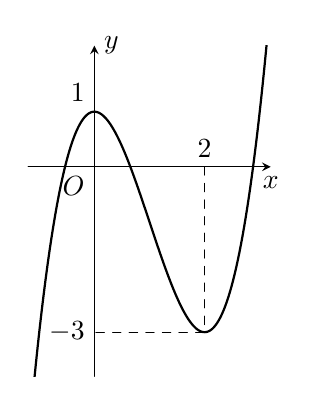
\begin{tikzpicture}[line cap=round, line join=round, >=stealth, scale=0.7]
			% Define plotting bounds
			\def\xmin{-1.2} \def\xmax{3.2}
			\def\ymin{-3.8} \def\ymax{2.2}
			
			% Scope clipping for graph drawing
			\begin{scope}
				\clip (\xmin,\ymin) rectangle (\xmax,\ymax);
				% Cubic curve y = x^3 - 3*x^2 + 1
				\draw[thick, smooth, samples=200, domain=\xmin:\xmax] 
				plot(\x, {(\x)^3 - 3*(\x)^2 + 1});
			\end{scope}
			
			% Dashed projection lines for local minimum (2, -3)
			\draw[dashed, thin] (2,0) -- (2,-3) -- (0,-3);
			
			% Axes
			\draw[->] (\xmin,0) -- (\xmax,0) node[below]{$x$};
			\draw[->] (0,\ymin) -- (0,\ymax) node[right]{$y$};
			
			% Key Labels and Origin
			\node[below left] at (0,0) {$O$};
			\node[above left] at (0,1) {$1$};
			\node[above] at (2,0) {$2$};
			\node[left] at (0,-3) {$-3$};
		\end{tikzpicture}
	\end{center}
	\begin{multicols}{4}
		\begin{enumerate}
			\item $N(2; -3)$.
			\item $M(0; 1)$.
			\item $x = 2$.
			\item $x = 0$.
		\end{enumerate}
	\end{multicols}
\end{baitap}
\begin{baitap}
	%đề 004		\textbf{Câu 9.}
	Giả sử giá trị nhỏ nhất của hàm số $y = x + e^{-2x}$ trên đoạn $[0; 2]$ là $a + \ln b$. Tính $ab$.
	\begin{multicols}{4}
		\begin{enumerate}
			\item $ab = \frac{\sqrt{2}}{2}$.
			\item $ab = \frac{1}{2}$.
			\item $ab = 1$.
			\item $ab = 2$.
		\end{enumerate}
	\end{multicols}
\end{baitap}

\begin{baitap}
	%đề 004		\textbf{Câu 10.} 
	Tính giới hạn $\lim\limits_{x \to (-1)^-} \dfrac{x - 2}{x + 1}$.
	\begin{multicols}{4}
		\begin{enumerate}
			\item $+\infty$.
			\item $-\frac{1}{2}$.
			\item $-\infty$.
			\item $1$.
		\end{enumerate}
	\end{multicols}
\end{baitap}

\begin{baitap}
Cho hàm số $y = f(x)$ liên tục trên đoạn $[-1; 3]$ và có bảng biến thiên như sau:
	\begin{center}
		
\begin{tikzpicture}[scale=.8]
			\tkzTabInit[lgt=1.5,espcl=3]{$x$/1, $y'$/1, $y$/2}{$-1$, $0$, $2$, $3$}
			\tkzTabLine{, +, 0, -, 0, +, }
			\tkzTabVar{-/$1$, +/$2$, -/$-2$, +/$3$}
		\end{tikzpicture}
	\end{center}
	Tìm giá trị nhỏ nhất của hàm số đã cho trên đoạn $[-1; 3]$.
	\begin{multicols}{4}
		\begin{enumerate}
			\item $2$.
			\item $3$.
			\item $-2$.
			\item $1$.
		\end{enumerate}
	\end{multicols}
\end{baitap}

\begin{baitap} 
	Cho hàm số $y = f(x)$ có đạo hàm $f'(x) = 3x^2(x-1)^3(x+2)^2, \forall x \in \mathbb{R}$. Số điểm cực trị của hàm số đã cho là
	\begin{multicols}{4}
		\begin{enumerate}
			\item $2$.
			\item $1$.
			\item $4$.
			\item $3$.
		\end{enumerate}
	\end{multicols}
\end{baitap}

\begin{baitap}
	Cho hàm số $y = \dfrac{ax^2 + bx + 1}{cx + 2}$ có đồ thị như hình vẽ bên dưới. Tính giá trị biểu thức $T = 2a + 3b - c$.
	\begin{center}
		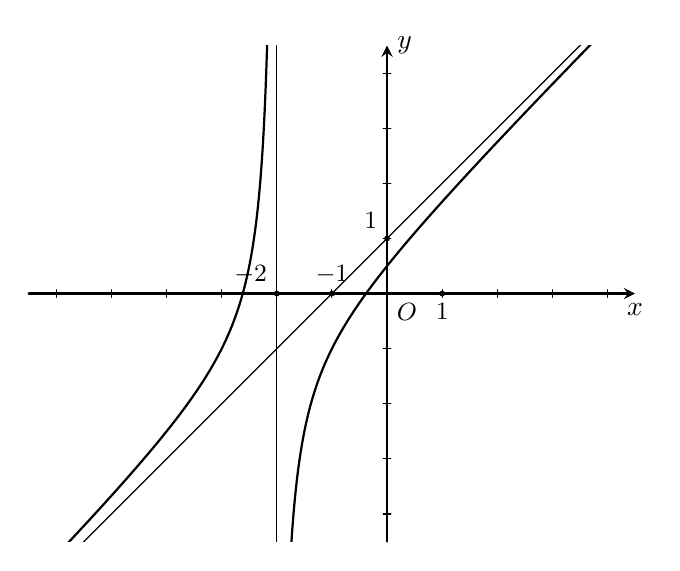
\begin{tikzpicture}[line cap=round, line join=round, >=stealth, scale=0.7]
			% Define coordinate window
			\def\xmin{-6.5} \def\xmax{4.5}
			\def\ymin{-4.5} \def\ymax{4.5}
			
			% Scope to clip the curve and asymptotes within viewing box
			\begin{scope}
				\clip (\xmin,\ymin) rectangle (\xmax,\ymax);
				
				% Asymptotes:
				% Vertical asymptote: x = -2
				\draw[black, thin] (-2,\ymin) -- (-2,\ymax);
				% Oblique asymptote: y = x + 1
				\draw[black, thin, domain=\xmin:\xmax] plot(\x, {(\x) + 1});
				
				% Graph of y = (x^2 + 3x + 1)/(x + 2) = x + 1 - 1/(x + 2)
				% Left branch: x < -2
				\draw[black, thick, smooth, samples=200, domain=\xmin:-2.08]
				plot(\x, {((\x)^2 + 3*(\x) + 1)/((\x) + 2)});
				
				% Right branch: x > -2
				\draw[black, thick, smooth, samples=200, domain=-1.92:\xmax]
				plot(\x, {((\x)^2 + 3*(\x) + 1)/((\x) + 2)});
			\end{scope}
			
			% Axes
			\draw[->, thick] (\xmin,0) -- (\xmax,0) node[below]{$x$};
			\draw[->, thick] (0,\ymin) -- (0,\ymax) node[right]{$y$};
			
			% Origin
			\node[below right, font=\small] at (0,0) {$O$};
			
			% Tick marks on x-axis
			\foreach \x in {-6,-5,-4,-3,-2,-1,1,2,3,4} {
				\draw (\x,2pt) -- (\x,-2pt);
			}
			
			% Tick marks on y-axis
			\foreach \y in {-4,-3,-2,-1,1,2,3,4} {
				\draw (2pt,\y) -- (-2pt,\y);
			}
			
			% Special point dots and labels as shown in original figure
			\fill (-2,0) circle (1.5pt) node[above left, font=\small] {$-2$};
			\fill (-1,0) circle (1.5pt) node[above, font=\small] {$-1$};
			\fill (1,0) circle (1.5pt) node[below, font=\small] {$1$};
			\fill (0,1) circle (1.5pt) node[above left, font=\small] {$1$};
			
		\end{tikzpicture}
	\end{center}
	\begin{multicols}{4}
		\begin{enumerate}
			\item $8$.
			\item $10$.
			\item $9$.
			\item $11$.
		\end{enumerate}
	\end{multicols}
\end{baitap}

\begin{baitap}
%	\textbf{Câu 1.} %đề 004
	Cho hình hộp chữ nhật $ABCD.A'B'C'D'$ có $AB = 4a$, $AD = 3a$, $AA' = 2a$ (tham khảo hình vẽ bên dưới). Gọi $\varphi$ là số đo góc nhị diện $[B, A'C', D]$. Tính $\tan \varphi$.
	\begin{center}
		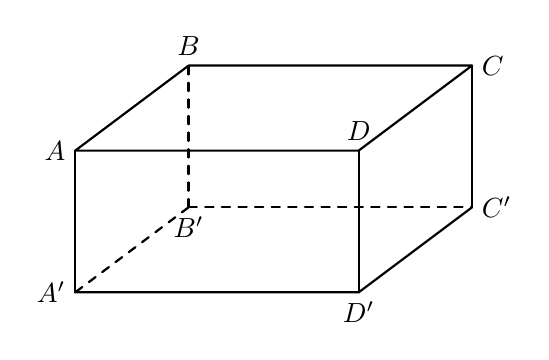
\begin{tikzpicture}[line cap=round, line join=round, >=stealth, scale=0.9]
			% Define 3D projection parameters manually for the rectangular cuboid
			% Top face vertices ABCD
			\coordinate (A) at (0, 2);
			\coordinate (B) at (1.6, 3.2);
			\coordinate (C) at (5.6, 3.2);
			\coordinate (D) at (4, 2);
			
			% Bottom face vertices A'B'C'D' (shifted downward)
			\coordinate (A') at (0, 0);
			\coordinate (B') at (1.6, 1.2);
			\coordinate (C') at (5.6, 1.2);
			\coordinate (D') at (4, 0);
			
			% Hidden edges (dashed)
			\draw[dashed, thick] (B') -- (A');
			\draw[dashed, thick] (B') -- (C');
			\draw[dashed, thick] (B') -- (B);
			
			% Visible edges of the cuboid (solid thick)
			\draw[thick] (A) -- (B) -- (C) -- (D) -- cycle;
			\draw[thick] (A') -- (D') -- (C');
			\draw[thick] (A) -- (A');
			\draw[thick] (D) -- (D');
			\draw[thick] (C) -- (C');
			
			% Vertex labels positioned relative to the projection
			\node[left] at (A) {$A$};
			\node[above] at (B) {$B$};
			\node[right] at (C) {$C$};
			\node[above] at (D) {$D$};
			\node[left] at (A') {$A'$};
			\node[below] at (B') {$B'$};
			\node[right] at (C') {$C'$};
			\node[below] at (D') {$D'$};
			
		\end{tikzpicture}
	\end{center}
	\begin{multicols}{4}
		\begin{enumerate}
			\item $-\frac{60}{11}$.
			\item $\frac{60}{11}$.
			\item $-\frac{40}{9}$.
			\item $\frac{40}{9}$.
		\end{enumerate}
	\end{multicols}
\end{baitap}

\begin{baitap}
%đề 004	\textbf{Câu 2.} 
Hai xạ thủ độc lập bắn vào một mục tiêu. Xác suất trúng mục tiêu của xạ thủ thứ nhất là $0{,}75$. Xác suất trúng mục tiêu của xạ thủ thứ hai là $0{,}85$. Xác suất để mục tiêu bị bắn trúng là
	\begin{multicols}{4}
		\begin{enumerate}
			\item $\frac{13}{40}$.
			\item $\frac{77}{80}$.
			\item $\frac{3}{5}$.
			\item $\frac{51}{80}$.
		\end{enumerate}
	\end{multicols}
\end{baitap}

\begin{baitap}
%đề 004	\textbf{Câu 3.} 
	Kết quả khảo sát cân nặng của 25 quả bơ được cho trong bảng sau
	\begin{center}
		\begin{tabular}{|c|c|c|c|c|c|c|}
			\hline
			Cân nặng ($\mathrm{gam}$) & $[150; 155)$ & $[155; 160)$ & $[160; 165)$ & $[165; 170)$ & $[170; 175)$ & $[175; 180)$ \\
			\hline
			Số quả & 2 & 4 & 7 & 8 & 3 & 1 \\
			\hline
		\end{tabular}
	\end{center}
	Tứ phân vị thứ ba (đơn vị: gam, kết quả làm tròn đến hàng phần chục) của mẫu số liệu trên bằng
	\begin{multicols}{4}
		\begin{enumerate}
			\item $Q_3 = 164{,}6$.
			\item $Q_3 = 168{,}6$.
			\item $Q_3 = 169{,}8$.
			\item $Q_3 = 160{,}2$.
		\end{enumerate}
	\end{multicols}
\end{baitap}

\begin{baitap}
%đề 004	\textbf{Câu 4.} 
	Tập nghiệm $T$ của bất phương trình $\log_{\frac{1}{3}}(x + 4) \ge -2$ là
	\begin{multicols}{4}
		\begin{enumerate}
			\item $T = (-4; 5]$.
			\item $T = (-4; 5)$.
			\item $T = [5; +\infty)$.
			\item $T = (-\infty; 5]$.
		\end{enumerate}
	\end{multicols}
\end{baitap}


\begin{baitap}
%đề 004	\textbf{Câu 6.} 
	Cho cấp số cộng $(u_n)$ có số hạng đầu $u_1 = -2$, công sai $d = 3$. Hỏi 199 là số hạng thứ mấy của cấp số cộng đã cho?
	\begin{multicols}{4}
		\begin{enumerate}
			\item 66.
			\item 67.
			\item 68.
			\item 69.
		\end{enumerate}
	\end{multicols}
\end{baitap}

\begin{baitap}
%đề 004	\textbf{Câu 7.} 
	Một nhà máy dự định sản xuất không quá 200 sản phẩm trong mỗi tháng. Biết giá bán của mỗi sản phẩm được tính theo hàm số $p(x) = 334 - \frac{3}{2}x$ (nghìn đồng), trong đó $x$ là số lượng sản phẩm sản xuất trong tháng. Hỏi mỗi tháng nhà máy đạt được doanh thu lớn nhất là bao nhiêu nghìn đồng \textit{(giả sử rằng các sản phẩm mà nhà máy sản xuất ra đều bán hết)}?
	\begin{multicols}{4}
		\begin{enumerate}
			\item $18592$.
			\item $18593$.
			\item $18592{,}7$.
			\item $18592{,}5$.
		\end{enumerate}
	\end{multicols}
\end{baitap}
\subsubsection*{Phần II. Thí sinh trả lời từ câu 1 đến câu 4, trong ý a), b), c), d) ở mỗi câu câu, thí sinh chọn ĐÚNG hoặc SAI.}
\setcounter{bt}{0}
\setlist[enumerate,1]{label=\quad\bfseries\alph*)}
\begin{baitap}
%Chuyên KHTN L1 25-26	\textbf{Câu 1.} 
	Một công ty sau khi ra mắt sản phẩm mới đã ghi nhận lợi nhuận $P(t)$ (đơn vị: tỷ đồng) sau $t$ tháng kinh doanh. Trong năm đầu tiên, giả sử mối liên hệ giữa lợi nhuận và thời gian kinh doanh được mô hình hóa bởi hàm số:
	\[
	P(t) = -t^3 + 12t^2 + 60t - 50, \quad 0 \le t \le 12.
	\]
	\begin{enumerate}
		\item Lợi nhuận của công ty tại thời điểm $t = 2$ là $110$ tỷ đồng.
		\item Hàm số biểu thị tốc độ tăng trưởng lợi nhuận $P'(t) = -3t^2 + 24t + 10$.
		\item Lợi nhuận của công ty đạt mức tối đa tại thời điểm $t = 10$.
		\item Tại thời điểm $t = 4$ thì tốc độ tăng trưởng lợi nhuận là lớn nhất.
	\end{enumerate}
\end{baitap}

\begin{baitap}
%Chuyên KHTN L1 25-26	\textbf{Câu 2.} 
	Cho hàm số $f(x) = \log_2(x^2 - 4x + 8)$.
	\begin{enumerate}
		\item Tập xác định của hàm số $f(x)$ là $D = \mathbb{R}$.
		\item Đạo hàm $f'(x) = \frac{2x - 4}{x^2 - 4x + 8}$.
		\item Giá trị nhỏ nhất của hàm số $f(x)$ trên $\mathbb{R}$ bằng $1$.
		\item Phương trình $f(x) = 2025$ có đúng hai nghiệm.
	\end{enumerate}
\end{baitap}

\begin{baitap}
%Chuyên KHTN L1 25-26	\textbf{Câu 3.} 
	Cho hàm số $y = \dfrac{2x^2 - x + 2}{x - 1}$ có đồ thị $(C)$.
	\begin{enumerate}
		\item Tập xác định của hàm số đã cho là $D = (1; +\infty)$.
		\item Hàm số đã cho có đúng hai điểm cực trị.
		\item Đồ thị $(C)$ có tiệm cận xiên là $y = 2x + 1$.
		\item Xét điểm $A$ thuộc $(C)$, tổng khoảng cách từ $A$ đến hai đường tiệm cận của $(C)$ luôn lớn hơn $2{,}3$.
	\end{enumerate}
\end{baitap}

\begin{baitap}
%Chuyên Bắc Ninh L1 25-26	\textbf{Câu 4.} 
	Cho hàm số $y = \left(9 - x^2\right)^{\frac{1}{3}} + \ln(1 - x)$
	\begin{enumerate}
		\item Tập xác định của hàm số là khoảng $(-\infty; 1)$.
		\item Hàm số có đạo hàm $y' = \dfrac{1}{3\sqrt[3]{(9 - x^2)^2}} - \dfrac{1}{1 - x}$.
		\item Hàm số nghịch biến trên khoảng $(0; 1)$.
		\item Giá trị nhỏ nhất của hàm số trên đoạn $\left[\frac{1}{4}; \frac{1}{2}\right]$ bằng $\frac{1}{2}\sqrt[3]{70} - \ln(2)$.
	\end{enumerate}
\end{baitap}

\subsubsection*{Phần III. Thí sinh trả lời từ câu 1 đến câu 6 (không làm tròn các phép tính trung gian trong các câu từ 1 đến câu 6).}
\setcounter{bt}{0}
\begin{baitap}
	%	\textbf{Câu 2.}  HSG Hà Nội 26-27
	Một chất điểm chuyển động có phương trình chuyển động là $s(t) = -\frac{1}{2}t^2 + 20t$ (đơn vị: mét), với $t \ge 0$ (đơn vị: giây). Sau 8 giây tính từ khi chất điểm bắt đầu chuyển động, vận tốc tức thời của chất điểm bằng bao nhiêu mét/giây?
	%	\begin{traloi}
		%		\textbf{$12$}
		%		\[
		%		s'(t) = -t + 20
		%		\]
		%		$\Rightarrow s'(8) = -8 + 20 = 12$.
		%	\end{traloi}
\end{baitap}
\begin{baitap}
	%Chuyên KHTN L1 25-26	\textbf{Câu 3.} 
	Một nhà máy sản xuất và bán $x$ sản phẩm trong mỗi tháng. Chi phí sản xuất $x$ sản phẩm được cho bởi công thức $C = 10000 + 600x - 0{,}6x^2 + 0{,}004x^3$ (nghìn đồng). Biết giá bán của mỗi sản phẩm là $p = 1800 - 6x$ (nghìn đồng). Hỏi mỗi tháng nhà máy nên sản xuất bao nhiêu sản phẩm để lợi nhuận thu được là lớn nhất?
\end{baitap}

\begin{baitap} %đề 004 26-27 \textbf{Câu III} ($1{,}5$ điểm). 
	Trong công nghệ sinh học sản xuất vắc-xin, sự phát triển số lượng vi khuẩn nuôi cấy trong môi trường dinh dưỡng giới hạn được mô hình hóa bởi hàm số Logistic $N(t) = \frac{A}{1 + Be^{-kt}}$ (trong đó $N(t)$ là số lượng vi khuẩn (đơn vị: \textit{triệu con}) sau $t$ giờ nuôi cấy ($t \ge 0$) và $A, B, k$ là các hằng số dương). Tốc độ sinh trưởng của quần thể tại thời điểm $t$ được xác định bởi hàm $v(t) = N'(t)$ (đơn vị: \textit{triệu con/giờ}). Biết rằng: Số lượng vi khuẩn tối đa mà môi trường này có thể duy trì khi thời gian nuôi cấy đủ lớn (xem số lượng này bằng $\lim\limits_{t \to +\infty} N(t)$) là $500$ triệu con; Tại thời điểm ban đầu ($t = 0$) quần thể có $20$ triệu con; Sau $2$ giờ nuôi cấy, số lượng vi khuẩn đạt $100$ triệu con. Người nuôi cấy cần can thiệp thu hoạch sinh khối tại thời điểm tốc độ sinh trưởng $v(t)$ đạt giá trị cực đại $v_{\max}$. Hãy tính tốc độ sinh trưởng cực đại $v_{\max}$ (triệu con/giờ) \textit{(không làm tròn các kết quả trung gian, làm tròn kết quả sau cùng đến hàng đơn vị)}.
\end{baitap}
\begin{baitap}
%	\textbf{Câu 1.} HSG Hà Nội 26-27
	Xét $A$ và $B$ là hai biến cố của một phép thử. Biết rằng xác suất của các biến cố $\overline{A}$, $B$, $A \cap B$ lần lượt là $P(\overline{A}) = 0{,}7$; $P(B) = 0{,}6$ và $P(A \cap B) = 0{,}1$. Hỏi xác suất của biến cố $A \cup B$ bằng bao nhiêu?
%	\begin{traloi} \textbf{$0{,}8$}
%		\[
%		P(A \cup B) = P(A) + P(B) - P(A \cap B) = 1 - P(\bar{A}) + P(B) - P(A \cap B)
%		\]
%		$\Rightarrow P(A \cup B) = 1 - 0{,}7 + 0{,}6 - 0{,}1 = 0{,}8$.
%	\end{traloi}
\end{baitap}

\begin{baitap}
%	\textbf{Câu 7.} HSG Hà Nội 26-27
	Cho hình chóp $S.ABCD$ có đáy $ABCD$ là hình chữ nhật, $AB = a$, $AD = 2a$; cạnh bên $SA$ vuông góc với mặt phẳng đáy và $SA = 2a$. Gọi $\alpha$ là số đo của góc nhị diện $[S, BD, C]$. Hỏi $\cos \alpha$ bằng bao nhiêu?
\end{baitap}

\begin{baitap}
%	HSG Hà Nội 26-27\textbf{Câu 8.} 
	Tổng của tất cả các nghiệm của phương trình $2\log_2(x + 5) + \log_2 x^2 = 2\log_2 6$ bằng bao nhiêu?
\end{baitap}






